% Sección obligatoria 6: Análisis de Resultados
% Toda cifra cita su log en pruebas/ o la bitácora (bitacora_web.md).
% Figuras generadas por informes/p2/scripts/figuras.py a partir de pruebas/.
% Metas del P1 no medidas = "no evaluada".
\section{Análisis de Resultados}
\label{sec:resultados}

Hicimos todos los ensayos en banco, entre el 6 y el 13 de noviembre de 2026, con alteraciones controladas. Las figuras de esta sección son originales: el script \texttt{informes/p2/scripts/figuras.py} las genera leyendo directamente los archivos de \texttt{pruebas/} del repositorio (\url{https://github.com/flauts/Qwapmayu}) y además imprime las cifras citadas en el texto. Distinguimos lo \textbf{observado}, que consta en un log, de lo que vimos en el hardware sin dejar registro; esto último lo indicamos explícitamente.

\subsection{Matriz de validación: meta del P1 frente a lo medido}
\label{sec:matriz}

La Tabla~\ref{tab:matriz} retoma los doce ensayos del perfil P1 y compara cada meta con lo medido. ``Cumplido'' significa que la evidencia satisface la meta en las condiciones indicadas; ``parcial'', que probamos solo una parte; ``no evaluada'', que no hicimos el ensayo previsto.

{\footnotesize
\renewcommand{\arraystretch}{1.15}
\begin{longtable}{p{2.0cm} p{3.0cm} p{4.5cm} p{1.45cm} >{\raggedright\arraybackslash\scriptsize}p{3.7cm}}
\caption{Matriz de validación: meta del P1 frente a lo medido}
\label{tab:matriz} \\
\toprule
Ensayo & Meta del P1 & Resultado medido & Estado & Evidencia (\texttt{pruebas/}) \\
\midrule
\endfirsthead
\toprule
Ensayo & Meta del P1 & Resultado medido & Estado & Evidencia (\texttt{pruebas/}) \\
\midrule
\endhead
pH & Calibrar con buffers; respuesta coherente y detección del cruce del umbral & Calibración de 2 puntos sin buffers; agua de caño 7.1--7.2 (tira: 7); agua hervida 8.46 (tira: 7--8); error declarado $\pm 1$. Cruce del umbral no ensayado & Parcial & \ev{sensores_20261111_141425_comp_agua_llave.log}, \ev{sensores_20261111_132707_comp_agua_llave.csv} \\
TDS & Incremento reproducible y detección sobre el umbral & Base 160 $\pm$ 22 ppm; con sal 141--681 ppm y solicitud de captura en un ensayo; sin calibración absoluta & Parcial & \ev{sensores_20261111_202348_cal_tds_base.csv}, \ev{sensores_20261111_223040_cal_tds_base.csv} \\
Turbidez & Cambio reproducible respecto a la referencia, sin NTU & Disparo en 2 réplicas con maicena; $\Delta I_T$ del pico 0.516 y 0.515; evolución posterior distinta & Cumplido (disparo) & \ev{sensores_20261109_122710_.._r2.csv}, \ev{.._194826_.._r3.csv} \\
Temperatura & Error $\leq 1\,^{\circ}$C frente a un termómetro de referencia & Lecturas estables de 23.75--23.88~$^{\circ}$C; sin termómetro de referencia; a veces el sensor no responde hasta reiniciar el nodo & No evaluada & \ev{sensores_20261112_001134_cal_tds.csv}; \ev{nodo_20261113_182101.log} \\
Anomalía persistente & Una sola solicitud y registro trazable & Siete capturas con turbidez real: ev=1 y ev=2 (7 nov), ev=18 (12 nov, bomba desconectada) y ev=3 a ev=6 en el ensayo integral (13 nov): 3 ciclos $\to$ MUESTREANDO $\to$ CAPTURA\_ESTIMADA $\to$ BLOQUEADO & Cumplido & \ev{nodo_20261107_225307.log}; \ev{sensores_20261112_003250_cal_tds.log}, L672--687; \ev{nodo_20261113_182101.log}; \ev{nodo_20261113_200907.log} \\
Pico aislado & Cero activaciones de la bomba & Anomalía simulada durante un ciclo: el nodo siguió en ARMADO & Cumplido (simulado) & \ev{serial_20261108_133113.log}, L255--274 \\
Dato inválido & Canal marcado inválido sin captura ni afectar a los demás & Turbidez desconectada: validez 0x06 $\to$ 0x02 y regreso a 0x06, sin captura; el gateway deja de publicar \texttt{it} & Cumplido & \ev{serial_20261108_133113.log}, L318--336; \ev{gateway_20261112_171838_gw_centinelas.log} \\
Dosificación & 10 captaciones; media $100 \pm 10$ mL & 10 disparos de 5000 ms: 100 mL $\pm$ 2.5 mL cada uno (resolución del frasco) en la geometría G1 & Cumplido (en G1) & \ev{bomba_manual_20261108_171604_serie_dosificacion_G1_70cm_d60_h2cm.log}; en el ensayo integral, 100 mL medidos por nosotros (sin log) \\
Enclava\-miento & Tras captura y reinicio, bomba apagada y estado BLOQUEADO & Reinicio tras captura $\to$ BLOQUEADO; reinicio durante el bombeo $\to$ FALLO; rearme rechazado con anomalía & Cumplido & \ev{serial_20261108_133113.log}, L451--487, L523--569, L591--625; \ev{nodo_20261112_145419_wdt_B_bomba.log} \\
Desconexión & El muestreo local continúa sin LoRa ni Internet & Con el radio en FALLO\_RADIO la captura se completó; corte de Wi-Fi con cola 3 $\to$ 9 $\to$ 0, sin bomba & Parcial & \ev{serial_20261108_133113.log}, L528--533; \ev{gateway_20261110_163055.log} \\
Enlace LoRa & 100 tramas en varias posiciones; PDR $\geq 95$~\% & 147/147 (PDR 100~\%) en una posición interior a 1~m; latencia mediana 106~ms & Cumplido en 1 posición & \ev{nodo_20261110_005911_p7_1m_nodo.log}, \ev{gateway_20261110_005746_p7_1m_gw.log} \\
Protección eléctrica & Sin reinicios del ESP32 por conmutar la bomba & Seis bombeos con la bomba conectada sin reinicio: 2 el 7 nov (con diodo en la bomba) y 4 en el ensayo integral (bobina alimentada desde el HW-131 y capacitor de 220~$\mu$F, sin diodo en la bomba); al inicio el USB se desconectaba al conmutar (observación sin log) & Cumplido (en banco) & \ev{nodo_20261107_225307.log}; \ev{nodo_20261113_182101.log}; \ev{nodo_20261113_200907.log} \\
\bottomrule
\end{longtable}
}

\subsection{Sensores}
\label{sec:res_sensores}

\textbf{pH.} Sin soluciones buffer, obtuvimos la recta con dos puntos. El primero fue el conector BNC en cortocircuito, que la documentación del fabricante trata como equivalente a pH 7 con un error de hasta 0.3~\cite{ph_sen0169}; dio 1345~mV. El segundo fue vinagre diluido, que la tira indicadora marcó como pH 3; dio 341~mV. Resulta $\mathrm{pH} = 0.003984\,\mathrm{mV} + 1.6410$, unos 251~mV por unidad de pH. Como verificación, el agua de caño dio pH 7.2 frente a 7 en la tira, y el 12 de noviembre dio 7.10. El agua hervida en reposo dio 8.46, mientras la tira marcó entre 7 y 8. La lectura tardó entre 3 y 15 minutos en estabilizarse. Con dos puntos cuyo valor de referencia viene de una tira, la pendiente real no queda acotada. Por eso declaramos un error de $\pm 1$ pH y no hay compensación por temperatura. La meta del P1, una calibración con buffers, no se cumplió. La Fig.~\ref{fig:tiras_ph} muestra las tiras usadas como referencia.

\begin{figure}[htbp]
\centering
\begin{minipage}[b]{0.48\textwidth}
\centering
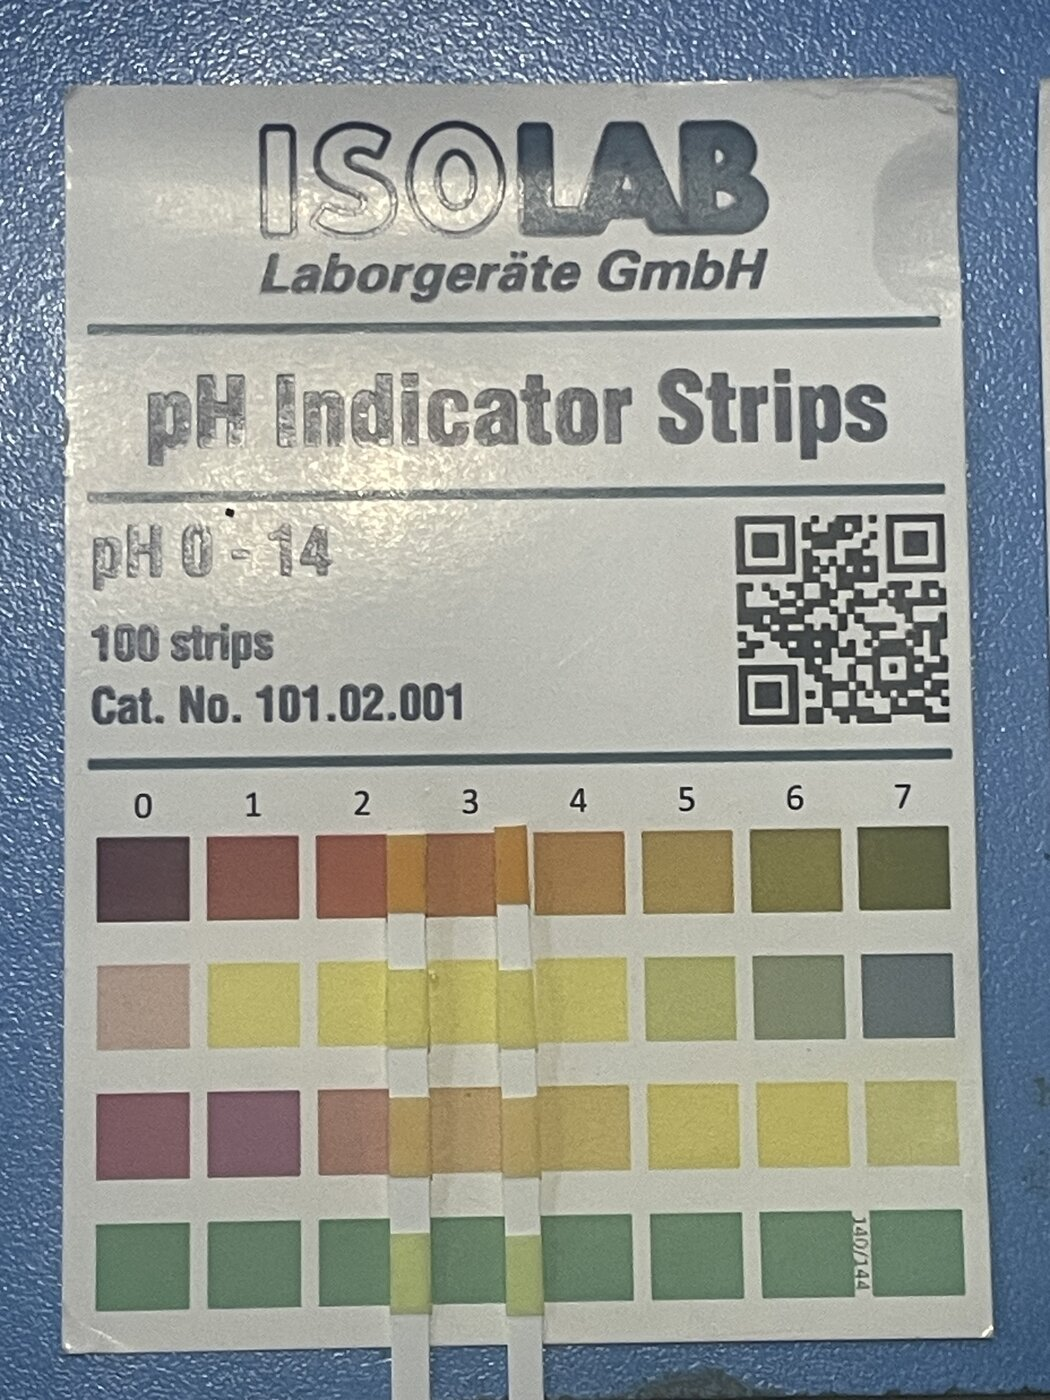
\includegraphics[width=\linewidth,height=7cm,keepaspectratio]{figuras/fotos/tira_ph_vinagre.jpg}\\
\small (a) Vinagre diluido: las tiras coinciden con la columna de pH 3 (punto B de la recta).
\end{minipage}\hfill
\begin{minipage}[b]{0.48\textwidth}
\centering
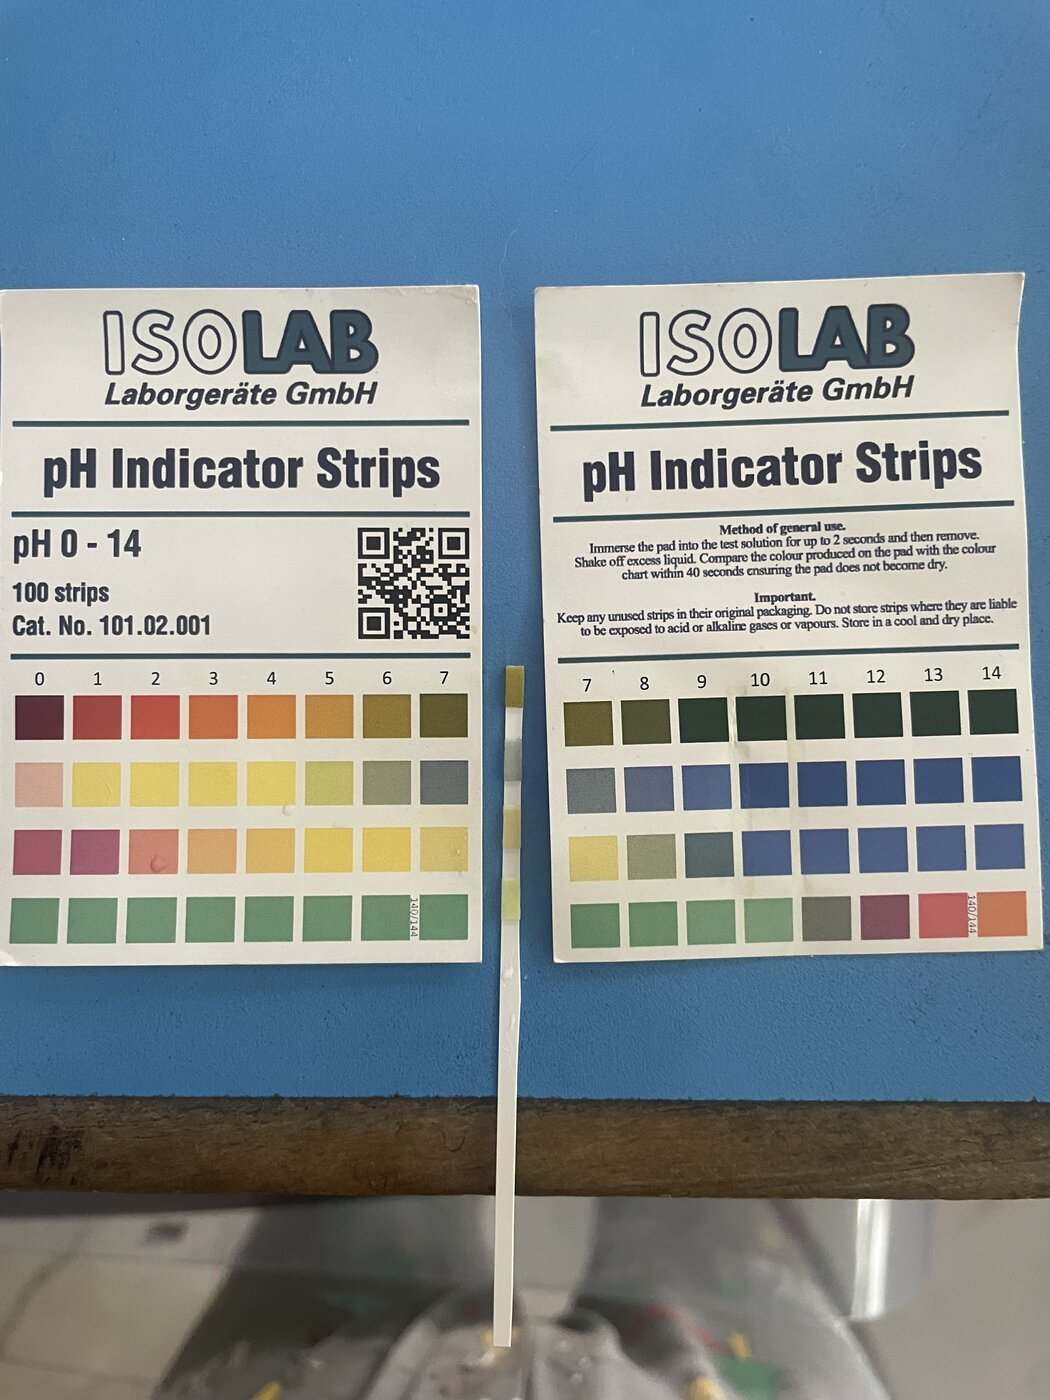
\includegraphics[width=\linewidth,height=7cm,keepaspectratio]{figuras/fotos/tira_ph_agua_cano.jpg}\\
\small (b) Agua de caño: la tira marca alrededor de pH 7; el sensor midió 7.2.
\end{minipage}
\caption{Tiras indicadoras de pH (ISOLAB, 0--14) comparadas con la escala del fabricante. La lectura de una tira es visual y tiene una resolución de una unidad de pH, por eso el error declarado del sensor es de $\pm 1$. Elaboración propia.}
\label{fig:tiras_ph}
\end{figure}

\textbf{TDS.} En agua de caño la línea base fue 160~ppm de media, con desviación de 22~ppm y un rango de 105 a 236~ppm en 897 lecturas (Fig.~\ref{fig:r2}a). Esa dispersión llevó a fijar el umbral 100~ppm sobre $TDS_0$. Una solución madre diluida casi no movió la lectura (de 0 a 10~ppm más). Una cucharada de sal seca en 500~mL, en cambio, la llevó hasta 681~ppm y activó la solicitud de captura (Fig.~\ref{fig:r2}b). En ese registro, $TDS_0$ había quedado en 114~ppm porque la versión de entonces tomaba una sola lectura. Tras un reinicio, la misma versión fijó $TDS_0$ en 566~ppm con el agua ya salada, lo que subió el umbral a 666~ppm y ocultó la anomalía. Este defecto motivó el cambio a la mediana de 12 lecturas tomadas después de 60~s. No contrastamos el KS0429 con un patrón, así que sus valores absolutos no están calibrados. Además, con la sonda desconectada el canal lee 58~ppm y se marca como válido, porque el TDS no tiene piso de validez.

\begin{figure}[htbp]
\centering
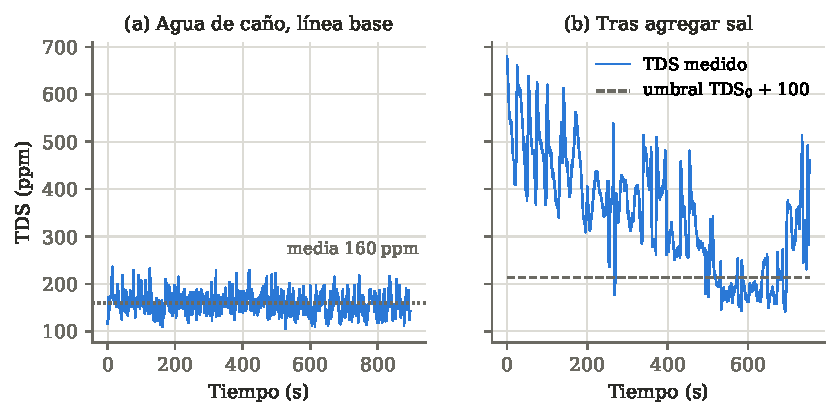
\includegraphics[width=\textwidth]{figuras/r2_tds.pdf}
\caption{TDS en agua de caño (a) y tras agregar sal (b). En (b), el umbral corresponde a $TDS_0 = 114$~ppm, fijado con una sola lectura por la versión anterior del firmware; graficamos el tramo previo al reinicio del registro. Fuentes: \texttt{pruebas/sensores\_20261111\_202348\_cal\_tds\_base.csv} y \texttt{pruebas/sensores\_20261111\_223040\_cal\_tds\_base.csv}. Elaboración propia.}
\label{fig:r2}
\end{figure}

\textbf{Turbidez.} La Fig.~\ref{fig:r1} superpone las dos réplicas con maicena, alineadas en el instante del disparo. En ambas el índice cruzó el umbral en pocos segundos después de agitar, y el pico quedó unos 0.52 por encima de la línea base: $\Delta I_T = 0.516$ en r2 y $0.515$ en r3. La línea base, sin embargo, fue distinta (0.019 y 0.073), y la evolución posterior también: r2 se mantuvo en una meseta cercana a 0.49, mientras que r3 se aclaró más rápido. Con dos réplicas y una cantidad de maicena no medida, el disparo se reproduce, pero no puede afirmarse que la magnitud se reproduzca. Observamos además tres limitaciones del sensor:
\begin{itemize}
    \item La maicena asentada en el fondo no activa el sensor: una réplica anterior con el sedimento ya depositado marcó $I_T \approx 0.10$ y solo disparó al agitar.
    \item En agua limpia, $I_T$ varió entre 0.013 y 0.058 según dónde colocamos el sensor.
    \item Sacar la sonda del agua produce 1 a 2~s de lectura falsa, que el filtro de tres ciclos absorbe.
\end{itemize}
Hicimos estos ensayos con el sensor en el pin de un montaje anterior. Repetimos el ciclo completo con el firmware final y los pines definitivos el 12 de noviembre, con $V_{T,0} = 2115$~mV y las cuatro sondas válidas (validez 0x0F). Al agitar la maicena, $I_T$ pasó de 0.133 a 0.357 y luego a 0.757 en ciclos sucesivos. Al tercer ciclo anómalo el nodo pasó a MUESTREANDO (evento 18), mantuvo el relé activo 5003~ms y quedó en BLOQUEADO. En esa prueba la bomba estaba desconectada, de modo que valida la lógica y la temporización, pero no el bombeo. Las capturas con la bomba conectada son las del 7 de noviembre (Fig.~\ref{fig:r4}) (\ev{sensores_20261112_003250_cal_tds.log}, L672--687; el archivo conserva la etiqueta de la prueba anterior, pero es la salida del nodo).

\begin{figure}[htbp]
\centering
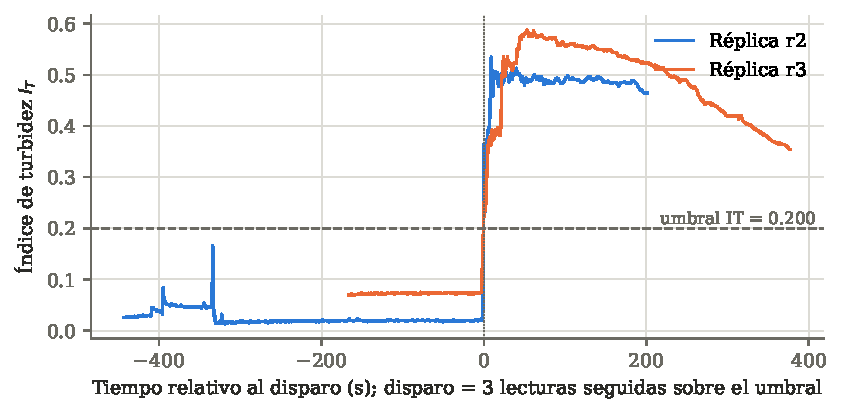
\includegraphics[width=0.85\textwidth]{figuras/r1_turbidez_maicena.pdf}
\caption{Índice de turbidez $I_T$ en las réplicas r2 y r3 con maicena, alineadas en el disparo (primera de tres lecturas seguidas sobre 0.200; lecturas cada 1 s). Fuentes: \texttt{pruebas/sensores\_20261109\_122710\_turb\_gpio4\_maicena\_r2.csv} y \texttt{pruebas/sensores\_20261109\_194826\_turb\_gpio4\_maicena\_r3.csv}. Elaboración propia.}
\label{fig:r1}
\end{figure}

\textbf{Temperatura.} El DS18B20 entregó lecturas estables, de 23.75 a 23.88~$^{\circ}$C en agua de caño (\texttt{sensores\_20261112\_001134\_cal\_tds.csv}). No lo contrastamos con un termómetro de referencia, así que la meta de error $\leq 1\,^{\circ}$C queda \textbf{no evaluada}. Además, observamos que a veces el sensor no responde y figura como desconectado hasta que se reinicia el nodo. Los registros del 13 de noviembre lo muestran en las dos sesiones del ensayo integral. En la de las 18:21, las 29 tramas previas al reinicio tienen la temperatura inválida y las 146 posteriores, válida. En la de las 20:09 son 96 inválidas antes del reinicio y 287 válidas después (\ev{nodo_20261113_182101.log}, \ev{nodo_20261113_200907.log}). En una tercera sesión, ese mismo día, el nodo no detectó el sensor ni siquiera después de reiniciar (\texttt{DS18B20=0} al arrancar; \ev{nodo_20261113_211917.log}). En cambio, durante los 87 minutos de la prueba de control del 12 de noviembre las 1045 tramas tuvieron temperatura válida. No determinamos la causa. El firmware inicializa el bus 1-Wire una sola vez, al arrancar (\texttt{nodo/src/main.cpp}), lo que es coherente con que el sensor solo se recupere reiniciando; un contacto intermitente en el cableado es otra explicación posible. Cuando la temperatura es inválida, el TDS se compensa con 25~$^{\circ}$C y la detección sigue funcionando, porque la temperatura no dispara capturas.

\subsection{Detección, captura y enclavamiento}
\label{sec:res_deteccion}

La Fig.~\ref{fig:r4} reconstruye, a partir de las tramas registradas, dos capturas reales provocadas con turbidez el 7 de noviembre, con la bomba conectada. En la segunda captura, la bomba se frenó por la tierra gruesa, pero el relé completó igualmente sus 5003~ms. En la primera, el índice superó 0.200 durante tres ciclos y el nodo pasó a MUESTREANDO. El relé estuvo activo 5003~ms (franja naranja), y luego el nodo pasó a CAPTURA\_ESTIMADA y a BLOQUEADO. Más de dos minutos después de la captura el índice llegó a 0.70, pero el nodo, ya bloqueado, no volvió a bombear; esto es justamente lo que debe hacer el enclavamiento. El rearme manual se aceptó solo después de tres ciclos normales, y la segunda alteración produjo una segunda captura idéntica. El ESP32 no se reinició en todo el registro.

\begin{figure}[htbp]
\centering
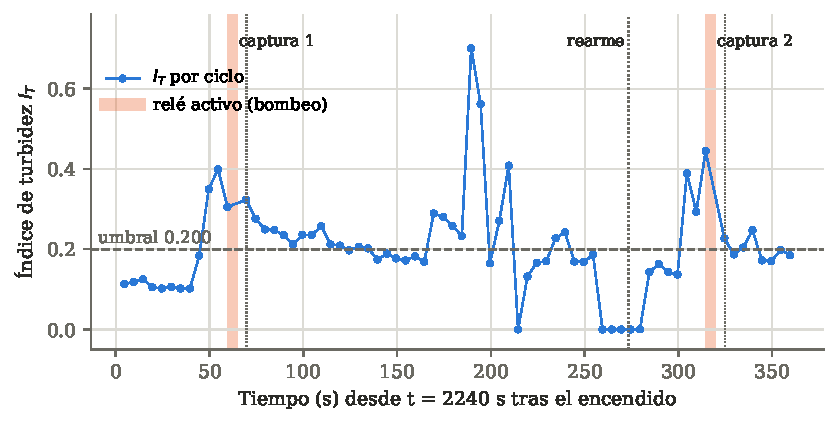
\includegraphics[width=0.9\textwidth]{figuras/r4_ciclo_estados.pdf}
\caption{Índice de turbidez por ciclo y estados del nodo durante dos capturas reales con la bomba conectada. $I_T$ se decodificó de cada trama transmitida; las franjas marcan el relé activo y las líneas punteadas, las transiciones a BLOQUEADO y el rearme. Fuente: \texttt{pruebas/nodo\_20261107\_225307.log}. Elaboración propia.}
\label{fig:r4}
\end{figure}

Probamos los casos de seguridad el 8 de noviembre con anomalías simuladas desde el teclado (\texttt{serial\_20261108\_133113.log}):
\begin{itemize}
    \item Con un fallo de NVS simulado, el nodo pasó a FALLO sin activar la bomba (L71--85).
    \item Una anomalía de un solo ciclo no produjo una captura (L255--274).
    \item Al desconectar el sensor de turbidez, su bit de validez pasó a 0 sin disparar nada (L318--336).
    \item El corte manual a los 406~ms de bombeo llevó a FALLO y vimos que la bomba se detuvo de inmediato (L386--399).
    \item Un reinicio con el botón EN durante el bombeo hizo arrancar en FALLO (L451--487).
    \item Un reinicio después de una captura hizo arrancar en BLOQUEADO (L523--569).
    \item El rearme se rechazó mientras persistía la anomalía y se aceptó tras tres ciclos normales (L591--625).
\end{itemize}

\textbf{\textit{Watchdog}.} Con un cuelgue provocado en reposo, el aviso del TWDT llegó a los 5.0~s y el nodo se reinició con motivo \texttt{TASK\_WDT}, volviendo a ARMADO (\texttt{nodo\_20261112\_145117\_wdt\_A\_ocioso.log}). Con el cuelgue justo después de encender el relé, el reinicio llegó unos 4.8~s después y el nodo arrancó en FALLO conservando el número de evento (\texttt{nodo\_20261112\_145419\_wdt\_B\_bomba.log}). En la prueba de control de unos 87 minutos, sin fallas forzadas, se transmitieron 1045 tramas sin saltos ni reinicios (\texttt{nodo\_20261112\_150625\_wdt\_control.log}). La captura completa que aparece en ese registro la provocamos con una anomalía simulada. En esta placa, el botón EN se reporta como \texttt{POWERON}, de modo que el motivo del reinicio no distingue un reinicio manual de un corte de energía.

\subsection{Dosificación}
\label{sec:res_dosif}

Hicimos la serie con la geometría G1: manguera de 70~cm y 6.5~mm de diámetro interior, 60~cm de tramo horizontal, boquilla 2~cm sobre el nivel de la fuente y 10~cm sobre la base del frasco, con la manguera vacía al inicio (Fig.~\ref{fig:foto_g1}). Usamos el firmware de banco \texttt{bomba\_manual}, en el que cada ensayo se inicia con el pulsador de GPIO25 y el relé se mantiene activo el tiempo pedido. Los diez disparos registraron \texttt{t\_pedido\_ms = t\_real\_ms = 5000} y terminaron con \texttt{motivo=normal} (líneas 20--38 del log). Leímos el volumen de cada disparo en un frasco con marcas cada 5~mL y fue de 100~mL en los diez casos, con una incertidumbre de $\pm 2.5$~mL por la resolución del frasco. La dispersión entre disparos fue menor que esa resolución, de modo que la meta de $100 \pm 10$~mL se cumplió en G1.

El volumen depende de la geometría. En pruebas previas, con una manguera de 30~cm obtuvimos unos 100~mL en 3.75 a 4.0~s, y con 70~cm y 30~cm de subida, 120~mL en 6~s y 160~mL en 8~s. Con la boquilla bajo el nivel de la fuente se formó un sifón que siguió vaciando la fuente con la bomba apagada. La manguera retiene unos 23~mL ($\pi \cdot 0.65^2/4 \cdot 70$~cm$^3$), que en cada disparo deben llenarse antes de que el agua llegue al frasco.

\subsection{Enlace LoRa, gateway y supervisión}
\label{sec:res_lora}

Con los módulos a 1~m en interior, en la ventana común de secuencias 143 a 289 el nodo envió 147 tramas y el gateway recibió las 147, es decir, un PDR del 100~\% (Fig.~\ref{fig:r3}). Suponiendo pérdidas independientes, la cota inferior del PDR con 95~\% de confianza es de aproximadamente 98~\%. La latencia, medida como la diferencia entre la marca de recepción y la de transmisión, fue de 104 a 107~ms con mediana de 106~ms. Esa cifra incluye el comando AT, el tiempo en el aire y el búfer del USB, y tiene un error de decenas de milisegundos. El RSSI estuvo entre $-37$ y $-34$~dBm y la SNR entre 12 y 13~dB. Fue una sola posición, sin registrar orientación ni obstáculos, así que no representa el alcance en campo. En una prueba anterior, el gateway validó una trama real, ignoró un duplicado y rechazó una trama alterada por CRC (\texttt{gateway\_20261108\_232333\_gw\_p5a\_boot.log}, L43 y L50).

\begin{figure}[htbp]
\centering
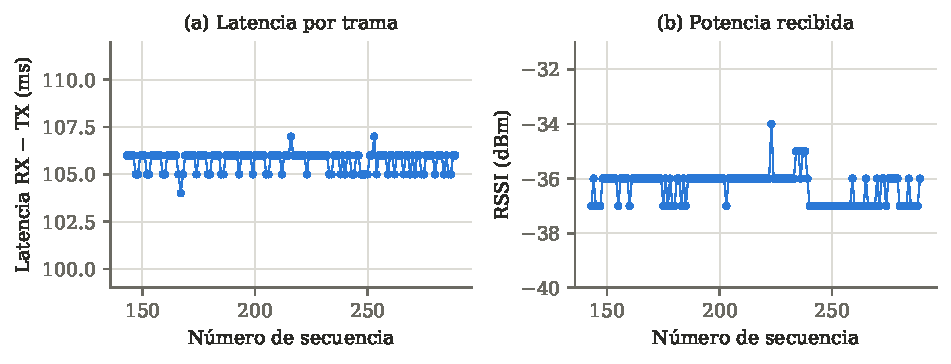
\includegraphics[width=\textwidth]{figuras/r3_lora.pdf}
\caption{Latencia (a) y RSSI (b) de cada trama del ensayo a 1~m; 147 de 147 tramas recibidas. Fuentes: \texttt{pruebas/nodo\_20261110\_005911\_p7\_1m\_nodo.log} y \texttt{pruebas/gateway\_20261110\_005746\_p7\_1m\_gw.log}. Elaboración propia.}
\label{fig:r3}
\end{figure}

\textbf{Corte de Internet.} Con el punto de acceso apagado, el gateway siguió recibiendo por LoRa (de 24 a 36 tramas acumuladas) mientras su cola pasaba de 3 a 9 mensajes. Al volver la conexión publicó todo y la cola volvió a 0 (\texttt{gateway\_20261110\_163055.log}, L32--56). La bomba no participó en este ensayo.

\textbf{Sordera del RAK.} El módulo receptor dejó de entregar tramas sin causa conocida al menos dos veces: el 8 de noviembre y el 9 de noviembre, esta vez durante unos 24~minutos hasta que pulsamos EN (\texttt{gateway\_20261109\_111821\_p6\_gw\_rx.log}). Con la recuperación automática, una sordera provocada se resolvió a los 60~s de silencio y el RX quedó rearmado en 1.57~s. Se perdieron las secuencias 20 a 31 y las 32 a 121 llegaron sin saltos (\texttt{gateway\_20261112\_165559\_gw\_sordera\_1.log}). Con el nodo apagado, el gateway hizo tres intentos y se reinició a los 240~s (\texttt{gateway\_20261112\_170626\_gw\_sordera\_2.log}). La recuperación limita la pérdida a unos 60~s de tramas, pero no elimina la causa.

\textbf{ThingsBoard (hasta el 12 de noviembre).} La cadena completa (nodo, LoRa, gateway, MQTT y ThingsBoard) entregó telemetría al dispositivo QM01 desde el 10 de noviembre, según vimos en el tablero. Con las cuatro sondas conectadas la validez fue 15. Al desconectar la turbidez bajó a 11 y la clave \texttt{it} dejó de publicarse, mientras la tarjeta conservaba el último valor. Con un pico de turbidez se activó la alarma de anomalía persistente (\texttt{gateway\_20261112\_171838\_gw\_centinelas.log}).

\subsection{Ensayo integral}
\label{sec:res_integral}

El 13 de noviembre hicimos el ensayo integral, en el domicilio de uno de los integrantes, con el firmware final, el radio en SF7 y la nueva cadena MQTT con el tablero propio (Fig.~\ref{fig:foto_integral}). El sensor de pH era prestado y ya se había devuelto, así que participaron tres sensores: TDS, turbidez y temperatura (validez 0x0E; 25.1 a 25.3~$^{\circ}$C). La bomba estuvo conectada y fuera del agua: el recipiente de prueba tiene una salida en su pared, cerca del fondo, y desde ahí un acople rápido alimenta por gravedad la entrada de la bomba, que impulsa el agua por la manguera hasta un balde colector (Figs.~\ref{fig:acople} y~\ref{fig:foto_integral}). Medimos 100~mL capturados; este volumen no consta en un log. Provocamos la anomalía agitando maicena en el recipiente del sensor de turbidez. No usamos ninguna anomalía simulada.

Hubo dos sesiones, con dos capturas cada una. La Fig.~\ref{fig:r5} muestra la primera:
\begin{itemize}
    \item El índice pasó de 0.115 a 0.357, 0.418 y 0.416 en ciclos sucesivos. Al tercer ciclo el nodo pasó a MUESTREANDO (evento 3), activó la bomba 5003~ms y quedó en BLOQUEADO.
    \item La turbidez siguió sobre el umbral varios minutos, pero el nodo bloqueado no volvió a bombear.
    \item Cuando el índice bajó, rearmamos el nodo, y una segunda alteración produjo el evento 4.
\end{itemize}
En la segunda sesión el ciclo se repitió con los eventos 5 y 6 ($I_T$ de 0.285 a 0.297 y de 0.217 a 0.230). Ninguno de los dos registros muestra un reinicio del ESP32 durante los cuatro bombeos (\ev{nodo_20261113_182101.log}, \ev{nodo_20261113_200907.log}).

La información de las cuatro capturas recorrió toda la cadena. El gateway recibió por LoRa las tramas de MUESTREANDO y de CAPTURA\_ESTIMADA con PDR del 100~\% y RSSI entre $-29$ y $-44$~dBm (\ev{gateway_20261113_182107.log}, \ev{gateway_20261113_200914.log}). El registrador del broker guardó los mensajes de \texttt{estado} y \texttt{evento} de las cuatro capturas, a las 18:26:16, 18:31:16, 20:23:49 y 20:27:19 (\ev{mqtt_20261113_182150.csv}). Entre las dos capturas de la primera sesión, el broker midió 299.957~s y el reloj del nodo 300.000~s: los eventos llegan al broker sin acumular retraso.

\begin{figure}[htbp]
\centering
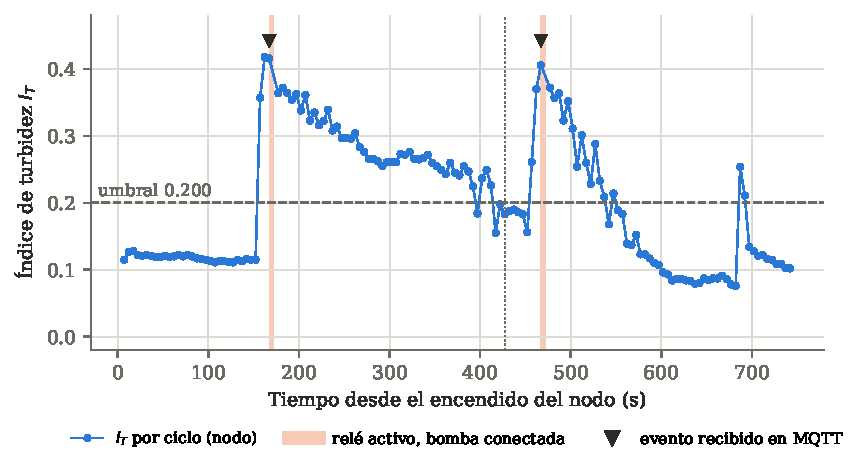
\includegraphics[width=0.92\textwidth]{figuras/r5_ensayo_integral.pdf}
\caption{Ensayo integral (primera sesión): índice de turbidez de cada trama, bombeos con la bomba conectada y llegada de cada evento al broker MQTT. Las marcas del broker se alinean en la primera captura; la segunda se ubica con el reloj del registrador. Fuentes: \texttt{pruebas/nodo\_20261113\_182101.log} y \texttt{pruebas/mqtt\_20261113\_182150.csv}. Elaboración propia.}
\label{fig:r5}
\end{figure}

\begin{figure}[htbp]
\centering
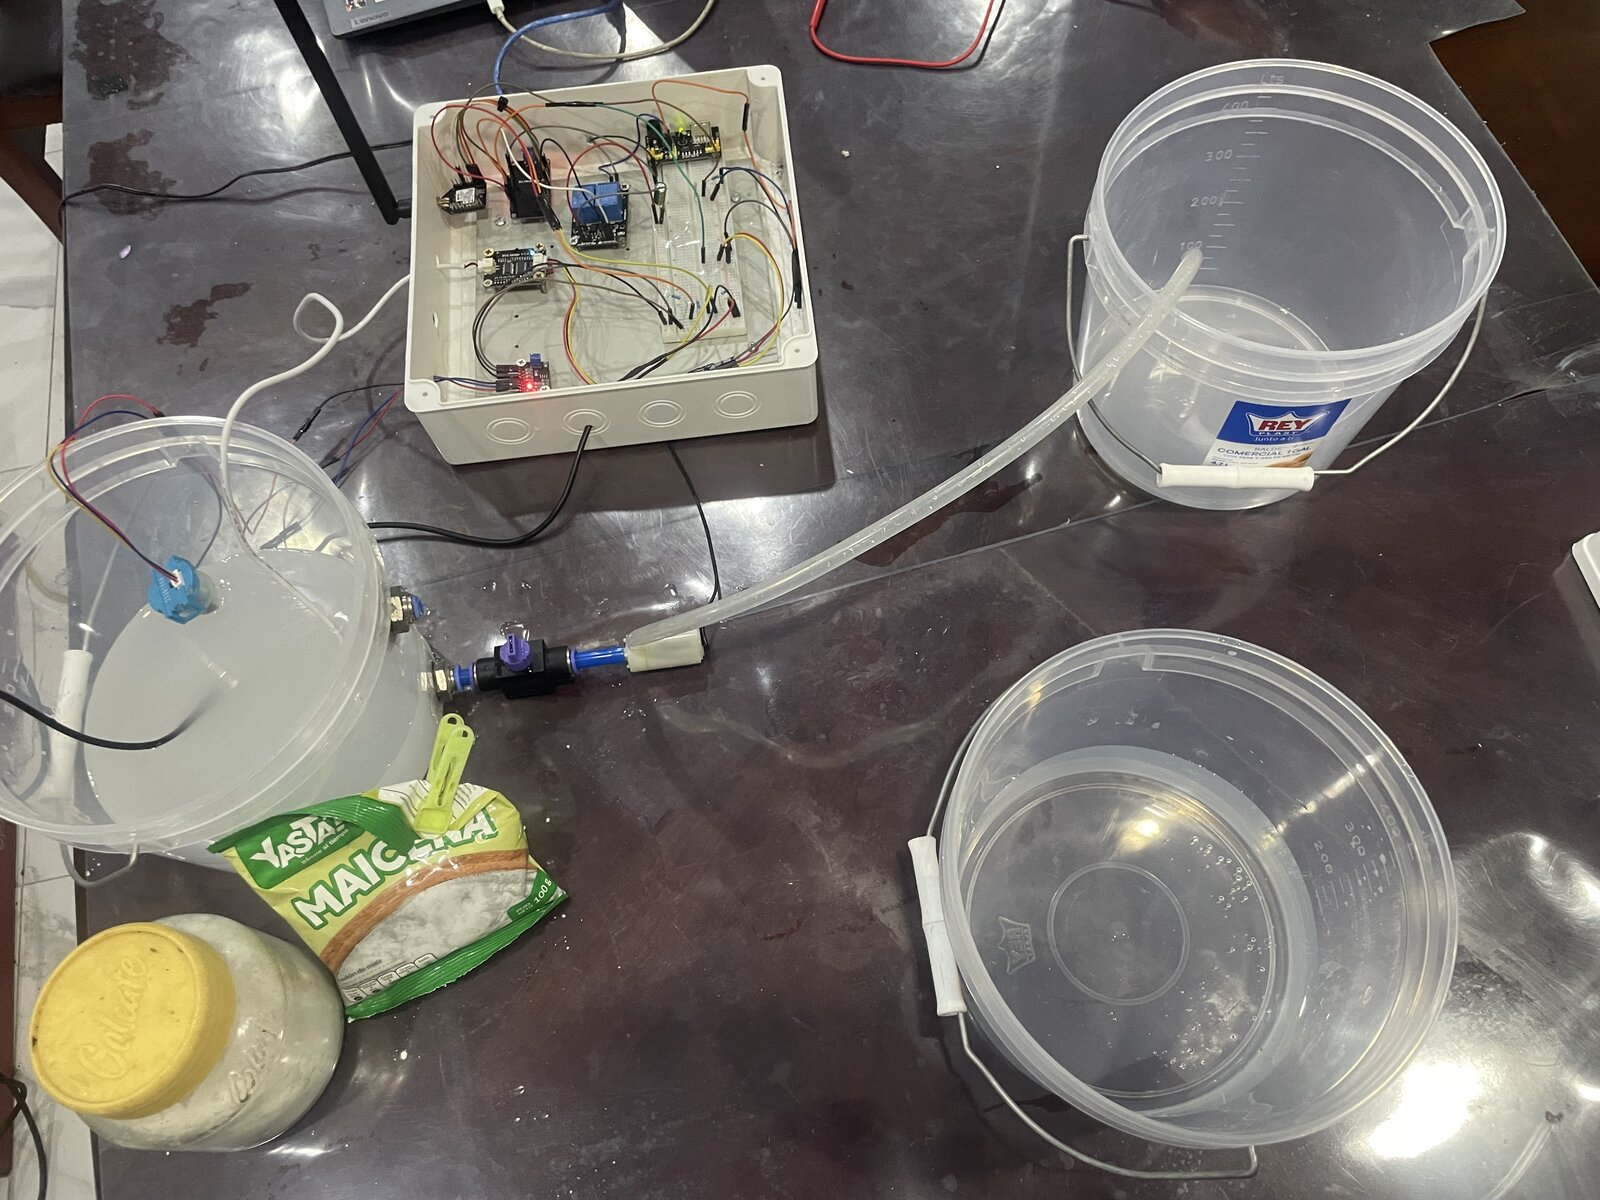
\includegraphics[width=0.6\textwidth]{figuras/fotos/ensayo_integral_montaje.jpg}
\caption{Montaje del ensayo integral, visto desde arriba. Abajo, el recipiente de prueba con los sensores y la maicena. De su pared sale el acople rápido hacia la bomba, que queda fuera del agua, y la manguera sube hasta el balde colector (arriba). A la izquierda, la caja del nodo. Fotografía tomada al terminar el ensayo. Elaboración propia.}
\label{fig:foto_integral}
\end{figure}
